The ECal uses an adapted version of the clustering algorithm that was used by the CLAS IC. The geometrical arrangement of the crystals differs greatly from that used by the IC and required detailed studies and simulations to reconstruct the incident particle energy. The angles of incidence of the particles (electrons, positrons, and photons) entering the Ecal varies significantly across the ECal. The edge effects in the ECal are substantial due to the horizontal split between the top and bottom halves and  the proximity to the beam. \\
\indent As a particle enters the ECal, it deposits all of its energy in the crystal material. Due to the segmentation of the calorimeter geometry, multiple adjacent crystals will contain some amount of the incident particle's energy. In offline clustering, the energy is reconstructed by summing all of the modules that measured some amount of the incident particle energy. The total reconstructed energy is always proportional to and less than the incident particle energy due to energy loss effects. These energy loss effects can be studied best through simulation and experimental testing with the electronics. 

\subsubsection{Simulations}
Simulations were performed using the fully modeled detector geometry in SLIC as part of the standard hps software package. The geometry includes all strips of the SVT, vacuum chambers, ECal crystals, and relevant dead material. The software also tracks particles through a 3D magnetic field map corresponding to the field values for 1~GeV beam running.~\cite{szumila-vance_hps_2016} \\
\indent Single electrons, positrons, and photons were simulated at discrete energies of 0.2, 0.3, 0.4, 0.5, 0.6, 0.7, 0.8,  0.9, 1.0, and 1.1~GeV to uniformly cover the ranger of energies detectable in the Engineering Run. The simulation uses the full reconstruction chain excluding pile-up effects. The offline cluster reconstruction uses the same thresholds used in data and production Monte Carlo: 7.5~MeV for individual hits, 50~MeV for seed hits in clusters, and 100~MeV for cluster energies.\\
\indent Due to the complex showering cascade that occurs when a particle deposits its energy in the ECal, several adjacent crystal modules contain some fraction of the incident energy of the particle. These modules are clustered in offline reconstruction to obtain the total deposited energy of the incident particle. The reconstructed energy $E_{rec}$ not corrected for shower loss effects is 

\begin{equation}
\label{eq:eclsum}
E_{rec} = \sum_i E_i    
\end{equation}

where $E_i$ is the energy of the $i^{\textrm{th}}$ module in the cluster. Some energy is lost between crystals and out the back of the ECal. After recovering the energy as measured by the ECal, the incident particle energy can be found by correcting for the shower loss effects as  

\begin{equation}
\label{eq:eclsf}
E_{corr} = \dfrac{E_{rec}}{f}   
\end{equation}

where $f$ is the energy-dependent ratio of measured vs incident particle energy. This factor is obtained through simulation by studying the reconstructed cluster energy against the known generated Monte Carlo particle energy. The energy loss corrections as derived from Monte Carlo are shown in Fig.~\ref{Figure:ecorr} where $E_{gen}$ refers to the simulated Monte Carlo particle energy.

\begin{figure}[thb]
  \centering
      \includegraphics[width=0.75\textwidth]{pics/performance/energycorrection.pdf}
  \caption[ECal energy shower correction functions derived from simulation]{The fraction $f$ is the reconstructed cluster energy, $E_{rec}$, divided by the Monte Carlo generated particle energy, $E_{gen}$ and is plotted versus the reconstructed energy. Each simulated particle type is shown in a different color, and the functional fit of Equation~\eqref{Figure:ecorr} for each particle is shown in dashed lines.}
  \label{Figure:ecorr}
\end{figure}

The difference in the energy corrections for the various particle types arises from geometrical effects and the incident angles of the particles entering the crystals.~\cite{szumila-vance_hps_ecal_2014} The focal point of the calorimeter, the point around which all crystals are angled, lies 80~cm from the front face of the ECal. The HPS target is beyond this focal distance at approximately 1.3~m from the face of the ECal and is offset beam right in the pair spectrometer magnetic field. Particles produced at the target take different trajectories from the target to the ECal due to the interactions of their charge and momentum in the magnetic field. This affects the entry angle of the particle into a crystal and mandates a charge and momentum-dependent energy correction function. The form of the energy correction function for the central region of the ECal is described by a three parameter fit.\\

\begin{equation}
	\label{eq:ecorrfunc}
	\dfrac{E_{rec}}{E_{gen}} = \dfrac{A}{E_{rec}}+\dfrac{B}{\sqrt{E_{rec}}}+C 
\end{equation}

The shower leakage effects in crystals becomes significant close to the calorimeter edge. The energy reconstruction deteriorates rapidly in the crystals closest to the edge but stabilizes in central region of the ECal. The energy reconstruction at the edges was characterized using Monte Carlo as a function of particle hit position in the ECal relative to the inner beam gap edge. In Equation ~\eqref{eq:ecorrfunc}, parameter $A$ is not strongly correlated with position and remains as a constant for a given particle type. The parameters $B$ and $C$  do depend on cluster position relative to the beam gap edge of the ECal. These dependencies can be seen for electrons in Fig.~\ref{Figure:sfparEdge}.

\begin{figure}[htb]
  \centering
      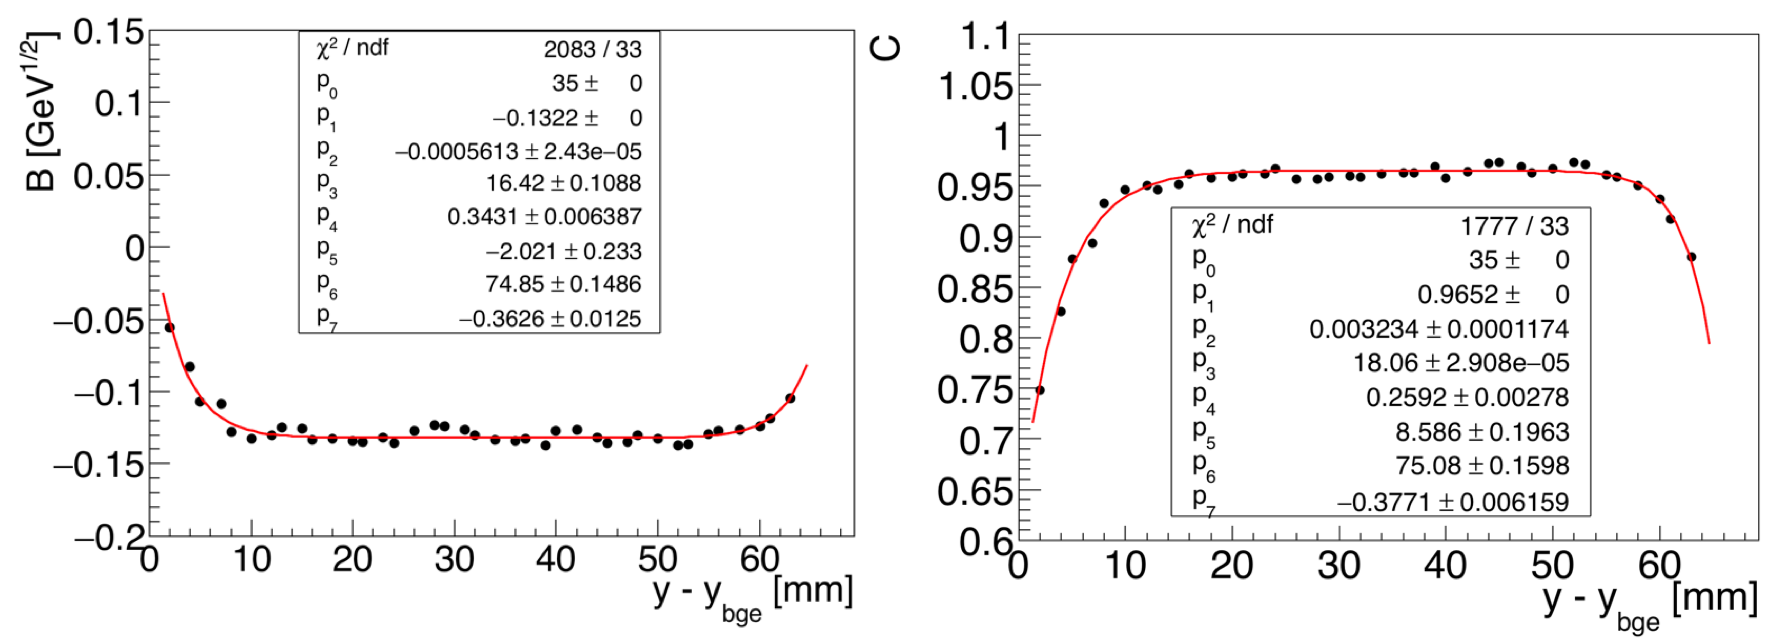
\includegraphics[width=1.0\textwidth]{pics/performance/sfparEdgeFit.png}
  \caption[ECal energy shower parameters for electrons relative to the inside beam gap edge]{Parameters $B$ and $C$ from Eq.~\ref{eq:ecorrfunc} for electrons, as a function of vertical position
relative to the innermost beam gap edge.}
  \label{Figure:sfparEdge}
\end{figure}

As shown in Fig.~\ref{Figure:sfparEdge}, the energy leakage parameters $B$ and $C$ can be fit with two functions at the edges that match in the central region of the ECal, away from the edges of the calorimeter. The equations used to fit the $B$ and $C$ parameters are described by:

\begin{equation}
\begin{split}
\label{eq:p1parlt}
B(y<p_0) = p_1-p_2 e^{-(y-p_3)p_4}\\
B(y>p_0) = p_1-p_5 e^{-(y-p_6)p_7}
\end{split}
\end{equation}

\begin{equation}
\begin{split}
\label{eq:p2parlt}
C(y<p_0) = p_1-p_2 e^{-(y-p_3)p_4}\\
C(y>p_0) = p_1-p_5 e^{-(y-p_6)p_7}
\end{split}
\end{equation}

The energy leakage correction functions are relatively constant in the central region of the calorimeter and are matched at a central distance $p_0$. For columns containing 5 crystals vertically, the distance to the beam gap edge is the absolute value of the distance from the cluster centroid to the innermost beam gap edge. In the regions above and below the region where row 1 crystals are removed in the ECal, additional consideration is made when calculating the distance to the inner beam gap edge in order to be consistent with other regions of the ECal. For completeness, the corresponding energy correction parameters for positrons and photons are seen in Figures~\ref{Figure:sfparEdgeEP} and \ref{Figure:sfparEdgeP}, respectively. 

\begin{figure}[htb]
  \centering
      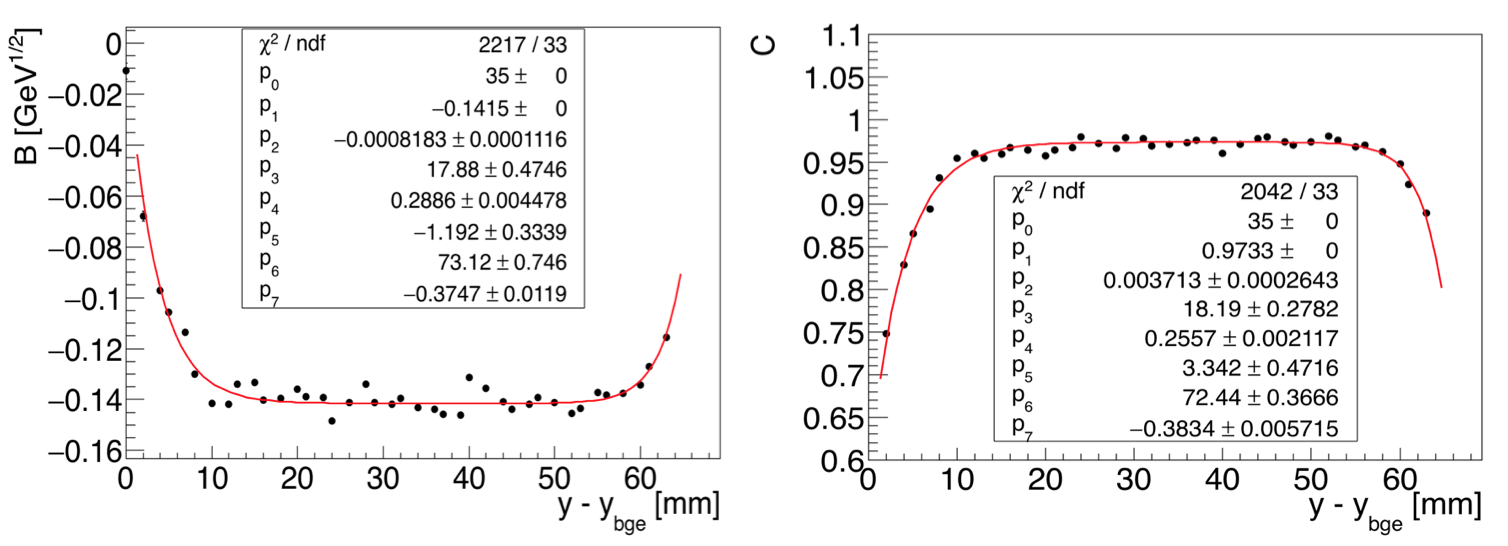
\includegraphics[width=1.0\textwidth]{pics/performance/sfparEdge_ep.png}
  \caption[ECal energy shower parameters for positrons relative to the inside beam gap edge]{Parameters $B$ and $C$ from Eq.~\ref{eq:ecorrfunc} for positrons, as a function of vertical position
relative to the innermost beam gap edge.}
  \label{Figure:sfparEdgeEP}
\end{figure}

\begin{figure}[htb]
  \centering
      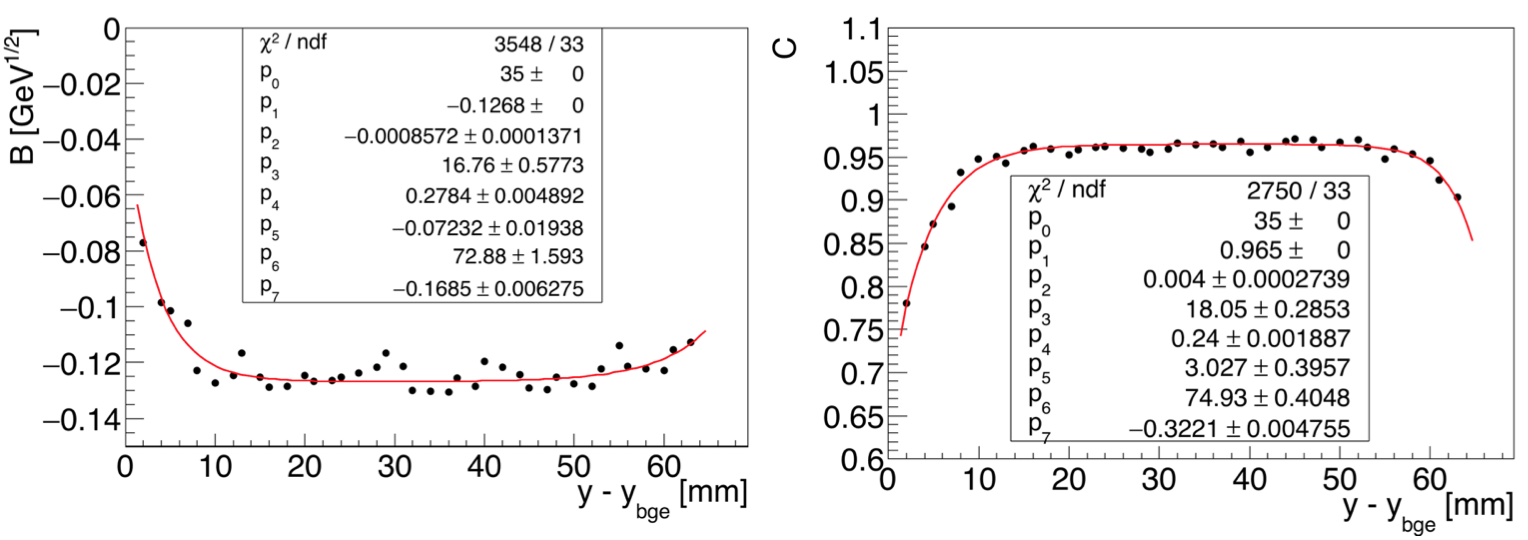
\includegraphics[width=1.0\textwidth]{pics/performance/sfparEdge_p.png}
  \caption[ECal energy shower parameters for photons relative to the inside beam gap edge]{Parameters $B$ and $C$ from Eq.~\ref{eq:ecorrfunc} for photons, as a function of vertical position
relative to the innermost beam gap edge.}
  \label{Figure:sfparEdgeP}
\end{figure}

As one can see, the energy correction fraction is relatively constant at approximately 1~cm from the edges of the ECal. As a result, we define the fiducial region of the ECal to be greater than 1~cm from the edge, or approximately 3/4 of the front face crystal dimension. This result is consistent with the findings for the CLAS IC~\cite{szumila-vance_hps_ecal_2014}.\\
\indent In reconstruction of the data, the energy of all the crystals in the cluster are summed to make the uncorrected, reconstructed cluster energy. Separately, tracks from the SVT are matched with clusters in the ECal. From the curvature of the track, the particle type can be determined as being either a positron or electron. Clusters that have no matching track are determined to be made from photons. The position of the track at the ECal and the particle type are used to apply the corrections in Equation~\eqref{eq:ecorrfunc} that contain the further edge corrections (if necessary) from Equations~\eqref{eq:p1parlt} and~\eqref{eq:p2parlt}. Photon clusters are corrected using the photon-type energy corrections and the position of the cluster in the ECal.  

\subsubsection{Energy resolution}

The energy resolution of the ECal is energy-dependent and improves with energy as approximately $1/\sqrt{E}$. From simulation, we obtain the energy resolution as shown in Figure~\ref{Figure:eResFitMC}.\\

\begin{figure}[htb]
  \centering
      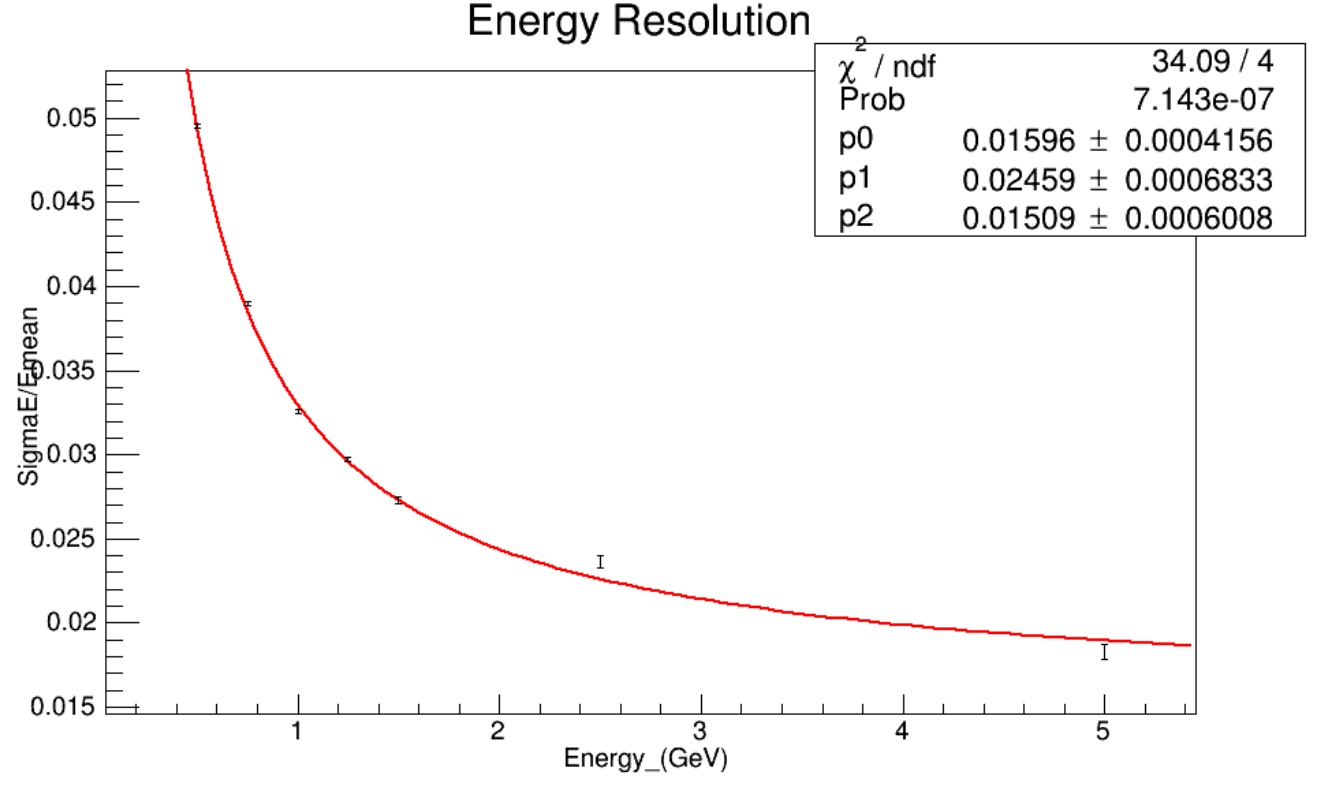
\includegraphics[width=0.6\textwidth]{pics/performance/eResFitMC.png}
  \caption[ECal fractional energy resolution fitted from simulation]{ECal fractional energy resolution from simulation. The points show the fractional energy resolution extracted from simulation, and the red line is the fit to the points.}
  \label{Figure:eResFitMC}
\end{figure}

The fit shown in Figure~\ref{Figure:eResFitMC} is described by 

\begin{equation}
\label{eq:eResMC}
\dfrac{\sigma_E}{E} (\%) = \dfrac{1.60}{E} \oplus \dfrac{2.46}{\sqrt{E}} \oplus 1.51
\end{equation}

The first term corresponds to the preamplifier noise. We were expecting 3~MeV$\times \sqrt{10} = 0.009$~GeV, where 10 is the average number of hit crystals, but we instead measured 0.016~GeV. This term from simulation is also not including the FADC error (expected to be 1.3~MeV~\cite{charles_2014}) which contributes a term (in $\%$) as $0.13\sqrt{10}/E$ which must be added quadratically. The second term corresponds to the statistical fluctuations in the shower development and is influenced by the lateral containment of the shower and energy deposited in the crystals. The second term from simulation does not include fluctuations in the number of photoelectrons (30 photoelectrons/MeV, multiplied by an excess noise factor parameterizing the fluctuations in the APD gain process, or Fano factor, of 2~\cite{panda_2008}) contributing $0.8/\sqrt{E}$. This term is calculated as $\sqrt{F/N_{pe/GeV}}$. The third term is interpreted as the fluctuation of energy leakage through the back of the crystals. This third term should include the crystal-to crystal inter-calibration error which is estimated to be 1~$\%$.~\cite{szumila-vance_hps_ecal_2014} By including these additional resolution effects in the measurement, we obtain the resolution as anticipated from Monte Carlo

\begin{equation}
\label{eq:eResUpdated}
\dfrac{\sigma_E}{E} (\%) = \dfrac{1.65}{E} \oplus \dfrac{2.59}{\sqrt{E}} \oplus 1.81 
\end{equation}

\subsubsection{Position reconstruction}
\indent ECal clusters can provide position information of comparable resolution to the SVT. Various weighting schemes for calculating a cluster centroid can be problematic due to periodic patterns resulting from the segmentation of the crystals. The same weighting scheme, used by the CLAS IC algorithm, provided the optimal position resolution. The calculation of the position of the cluster is~\cite{szumila-vance_hps_ecal_2014}

\begin{equation}
\begin{split}
\label{eq:posncalc}
x_{cl} & =  \dfrac{\sum_i w_i x_i}{\sum_i w_i}\\
y_{cl} & =  \dfrac{\sum_i w_i y_i}{\sum_i w_i}
\end{split}
\end{equation}

where $x_i$ and $y_i$ are the $x-$ and $y-$ positions of the $i^{\textrm{th}}$ crystal in the cluster, and $w_i$ is described by 

\begin{equation}
\label{eq:posnwt}
w_i  =  \max[0, w_0+\ln\dfrac{E_i}{E_{rec}}]
\end{equation}

Here $E_i$ is the energy deposited in the $i^{\textrm{th}}$ crystal, $E_{rec}$ is the sum of the energies of all of the crystals in the cluster, and $w_0$ is an energy threshold such that $E_i/E_{rec} > e^{-w_0}$ and is found in simulation to have a value of $3.1$~\cite{szumila-vance_hps_ecal_2014}. The logarithmic term enhances the contribution from the tails and improves the position measurement. Additional effects resulting from the differing angles of entry at the ECal require a position correction to the $x$-coordinate of the cluster. These corrections are both charge and momentum-dependent. The position correction for a generated 1~GeV electron is shown in Figure~\ref{Figure:xposn1gev}.

\begin{figure}[htb]
  \centering
      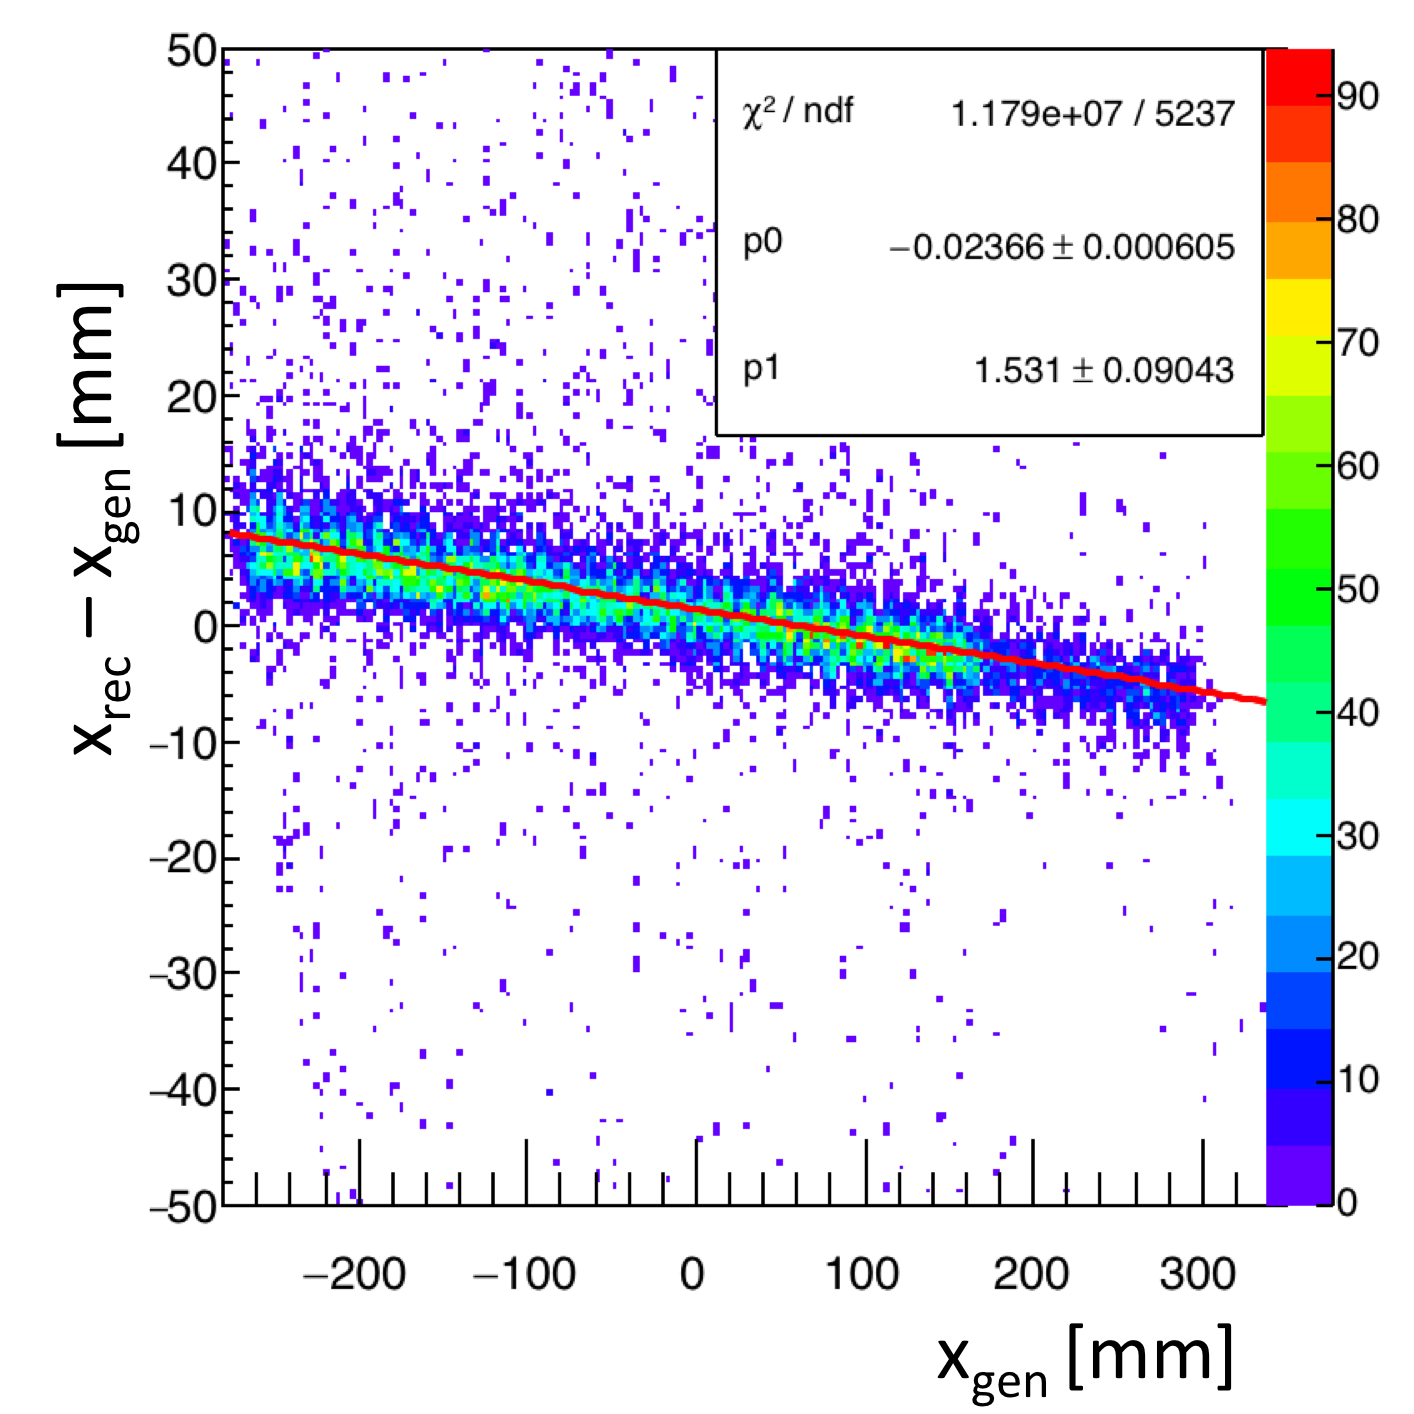
\includegraphics[width=0.7\textwidth]{pics/performance/xposn1gev.png}
  \caption[Horizontal position correction for 1~GeV electrons]{The position correction for 1~GeV electrons plotted versus the Monte Carlo generated position at the ECal. It is dependent both energy and position-dependent in order to account for the different angles of incidence at the ECal.}
  \label{Figure:xposn1gev}
\end{figure}

The correction at each energy by particle-type is fit with Equation~\eqref{eq:posncorr}. 

\begin{equation}
\label{eq:posncorr}
x_{rec} - x_{gen} = A(E_{rec}) x_{gen} + B(E_{rec})
\end{equation}

The energy-dependence of the fit parameters $A(E_{rec})$ and $B(E_{rec})$ use the reconstructed cluster energy, uncorrected for shower loss effects. These parameters for the electron horizontal position correction as a function of the reconstructed cluster energy are shown Figure~\ref{Figure:xposcorrPar}.

\begin{figure}[htb]
  \centering
      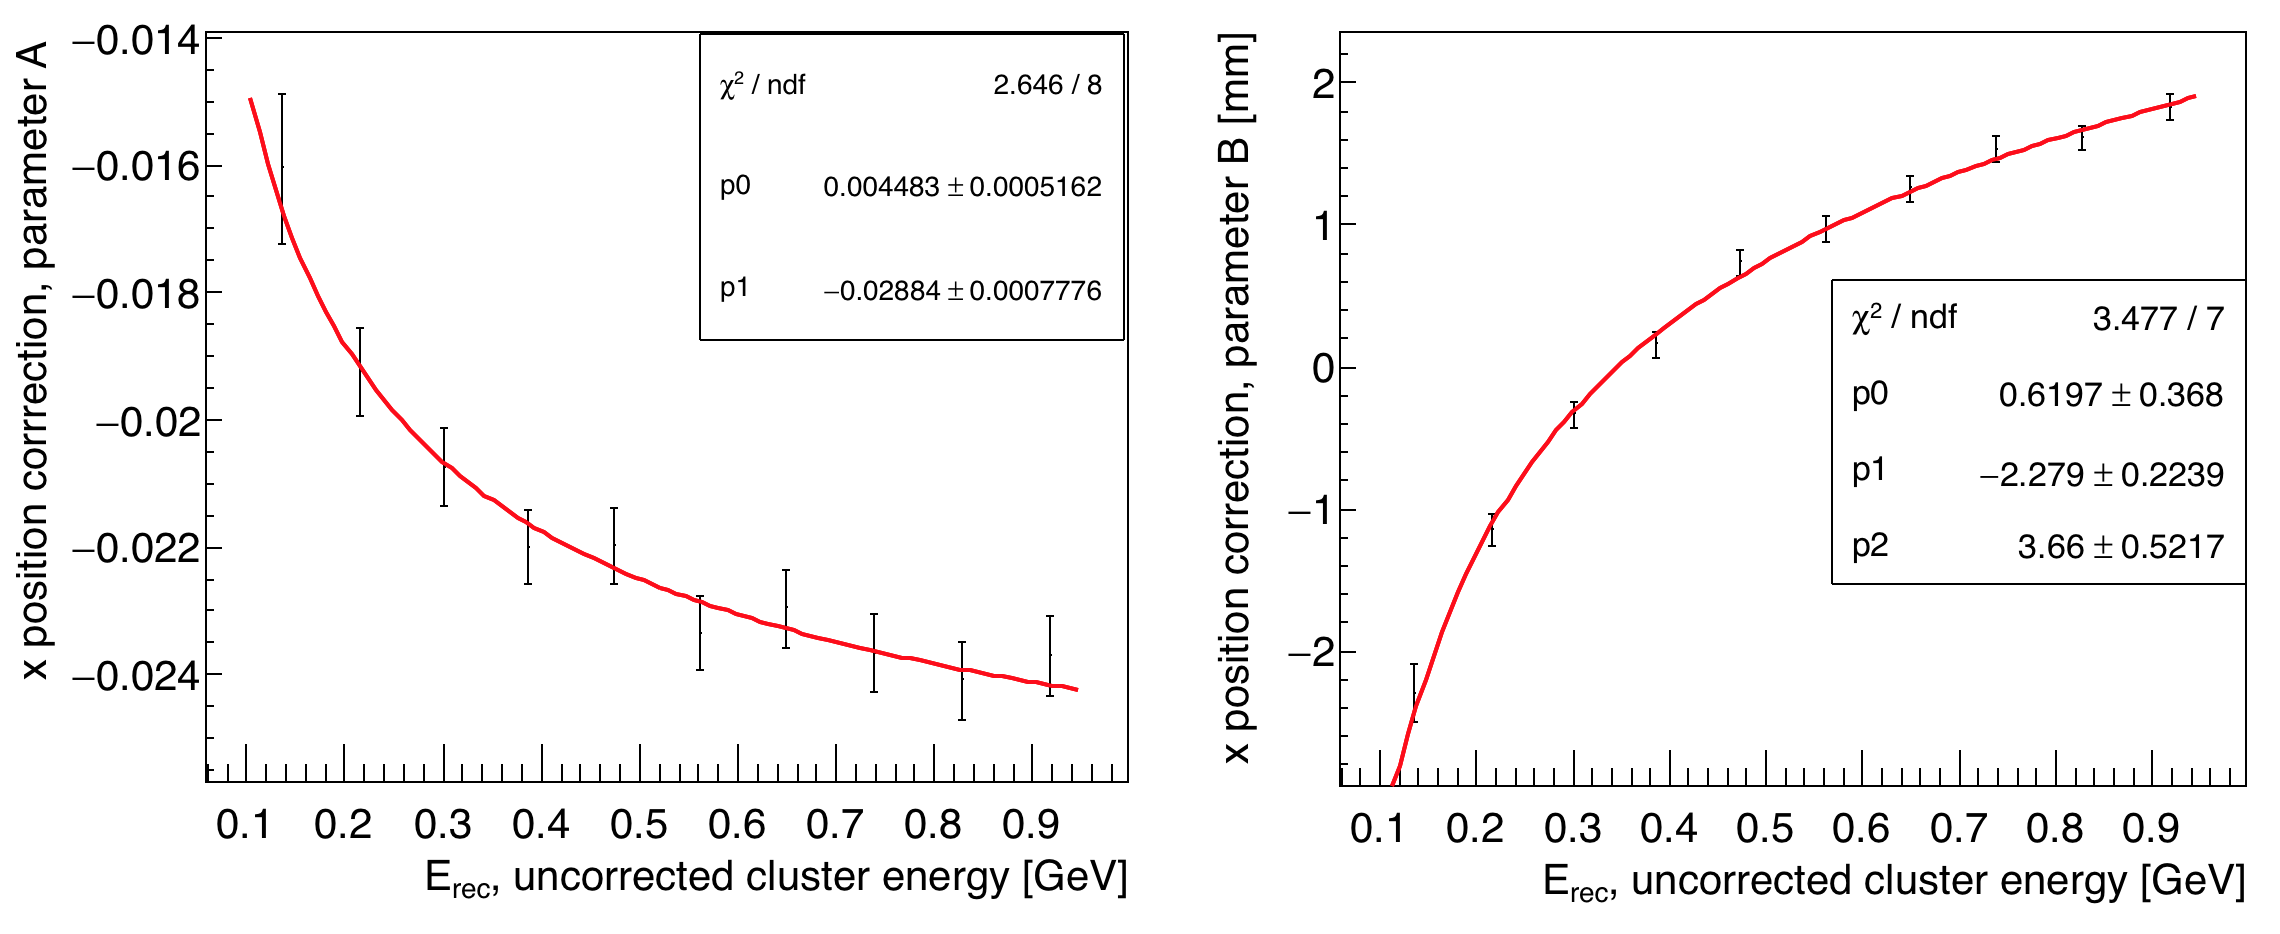
\includegraphics[width=1.0\textwidth]{pics/performance/xposcorrPar.png}
  \caption[Horizontal position correction dependence for electrons]{The horizontal position correction parameters as functions of the reconstructed cluster energy (without any further energy corrections for shower loss).}
  \label{Figure:xposcorrPar}
\end{figure}

The parameters in Figure~\ref{Figure:xposcorrPar} are fit to functions of the form described in Equation~\eqref{eq:posnCpar}.

\begin{equation}
\label{eq:posnCpar}
\begin{split}
A(E_{rec}) & =  \dfrac{p0}{\sqrt{E_{rec}}}+p1\\
B(E_{rec}) & =  p0\times E_{rec} +\dfrac{p1}{\sqrt{E_{rec}}}+p2
\end{split}
\end{equation}

The corresponding correction values for all three particle types can be summarized in Table~\ref{tab:horizPosCorr}.

\begin{table}[htb]
\caption{Horizontal position corrections.}
\label{tab:horizPosCorr}
\centering
\begin{tabular}{|c|c|c|}
\toprule
%\multicolumn{2}{c}{Name} \\
%\cmidrule(r){1-2}
Particle & $A(E_{rec})$ & $B(E_{rec})$ \\
\midrule
electron & $0.004483/\sqrt{E_{rec}}-0.02884$ & $0.6197E_{rec}-2.279/\sqrt{E_{rec}}+3.66$ \\
positron & $0.006887/\sqrt{E_{rec}}-0.03207$ & $-0.8048E_{rec}+0.9366/\sqrt{E_{rec}}+2.628$ \\
photon & $0.005385/\sqrt{E_{rec}}-0.03562$ & $-0.1948E_{rec}-0.7991/\sqrt{E_{rec}}+3.797$ \\
\bottomrule
\end{tabular}
\end{table}

Position corrections are not needed for the vertical cluster position.

\subsubsection{Position resolution}

After applying the position corrections to each particle-type at the simulated energies, the residual between the measured and simulated position reconstruction is obtained. The fitted residuals after correcting the position of 1~GeV electron clusters are shown in Figure~\ref{Figure:corrPosnsFits}.

\begin{figure}[htb]
  \centering
      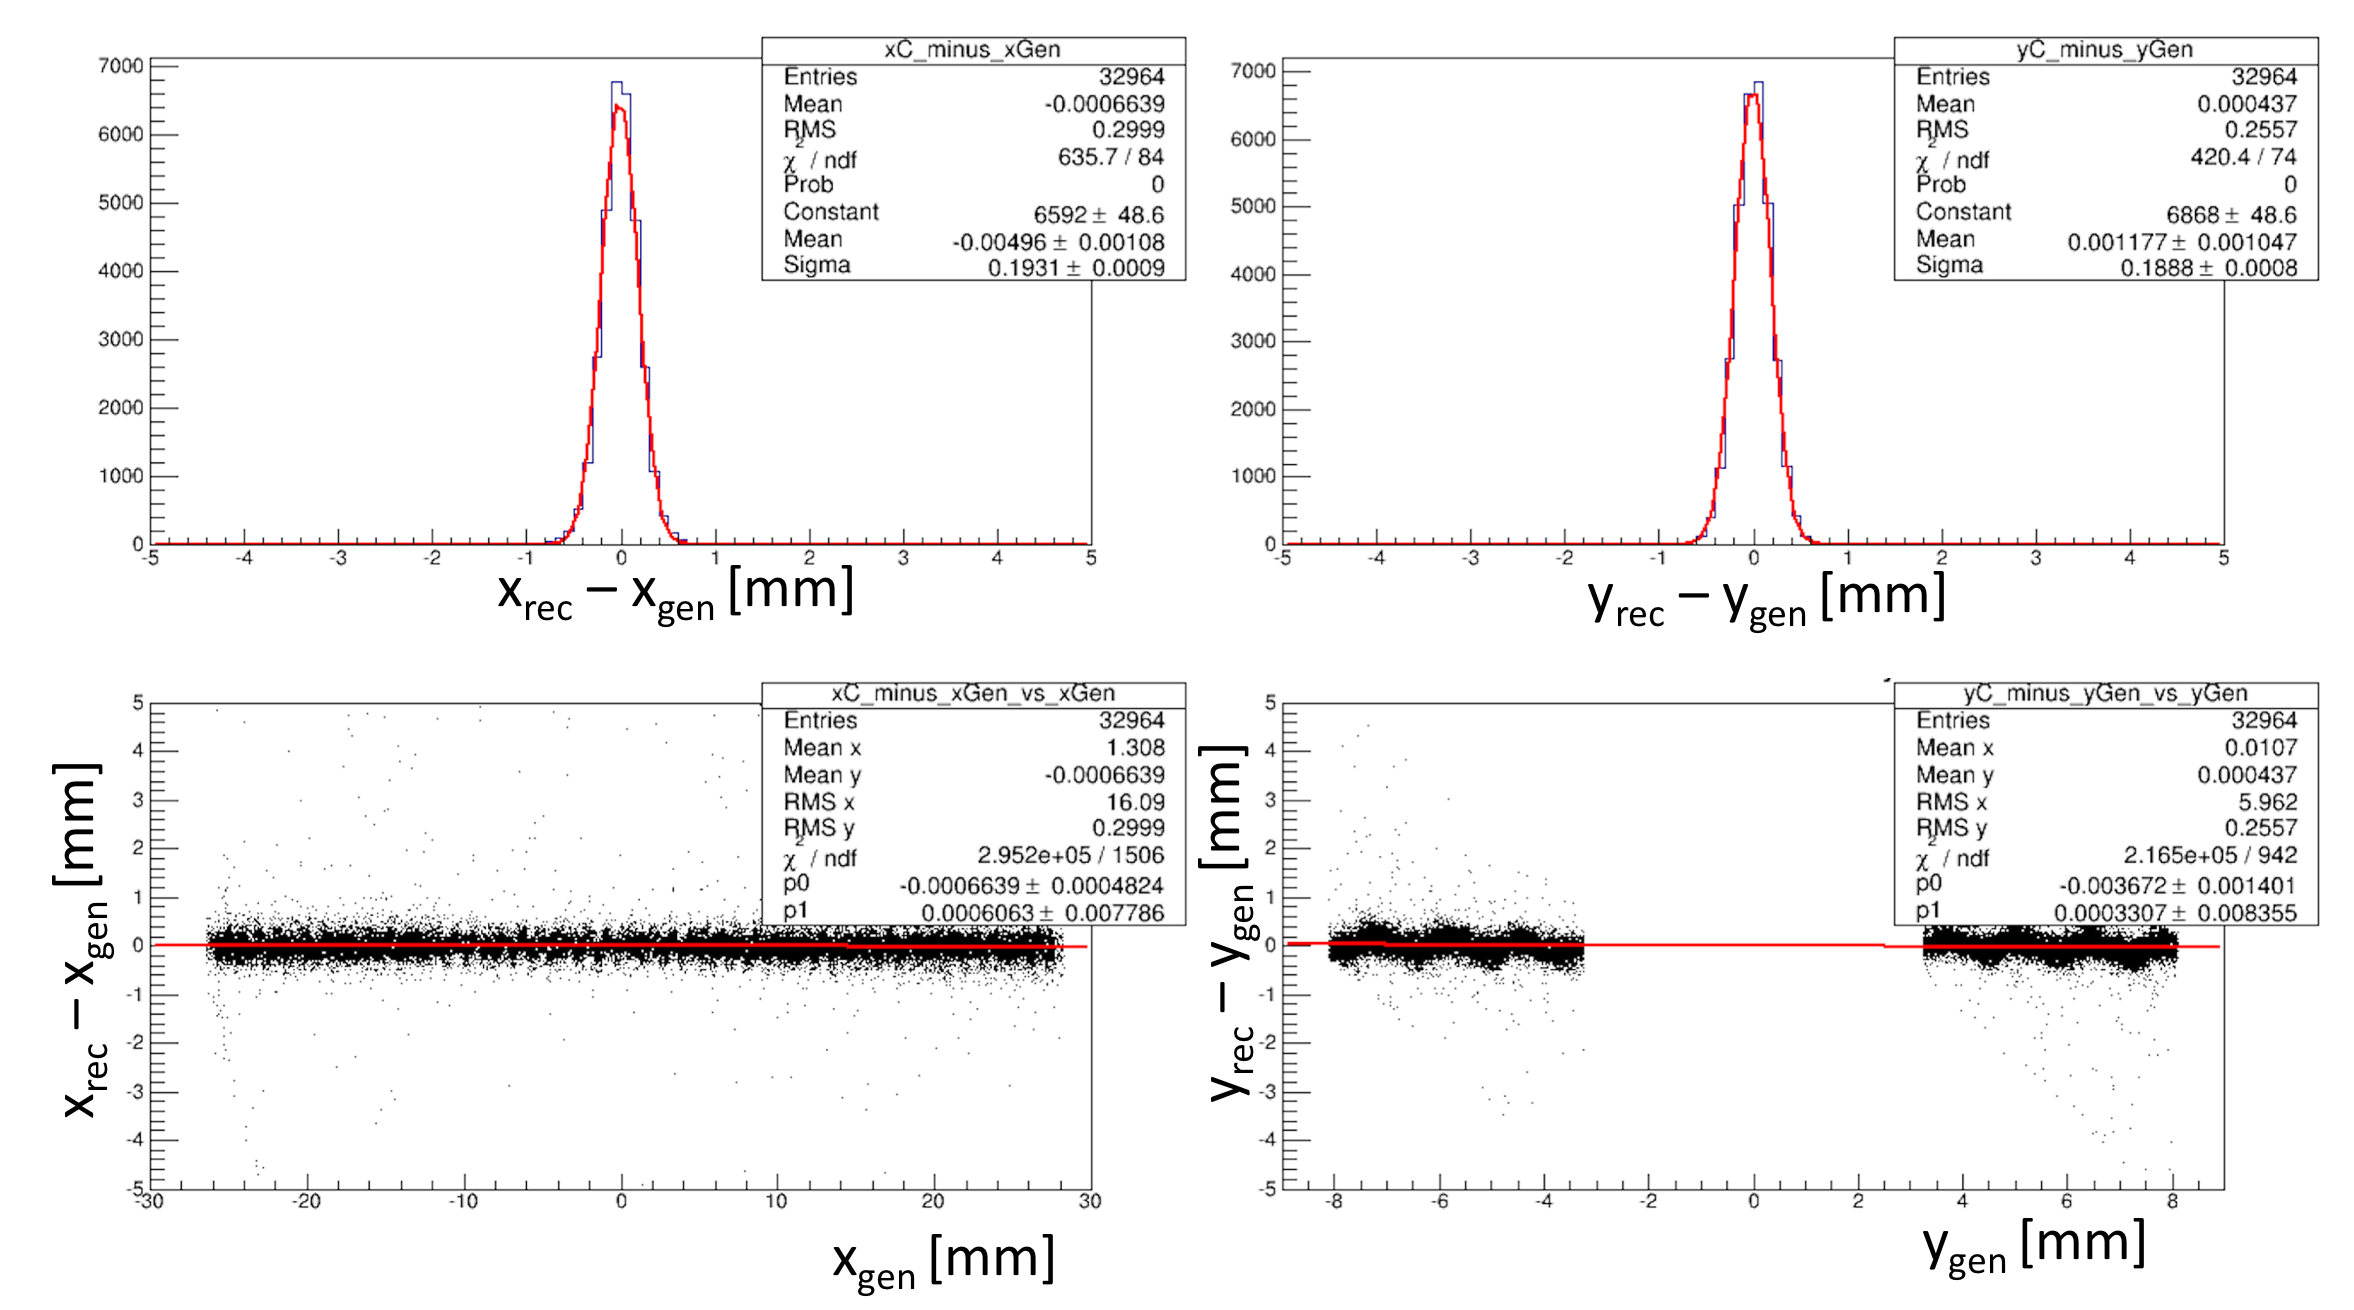
\includegraphics[width=1.0\textwidth]{pics/performance/corrPosnsFits.png}
  \caption[Position resolution for 1~GeV electrons.]{The position resolution for 1~GeV electrons, after applying the horizontal position corrections.}
  \label{Figure:corrPosnsFits}
\end{figure}

As shown in Figure~\ref{Figure:corrPosnsFits}, no correction is required when reconstructing the vertical position of the cluster. The energy-dependent resolution of both the horizontal and vertical position of reconstructed clusters can be seen for electrons in Figure~\ref{Figure:emPosnResn}. 

\begin{figure}[htb]
  \centering
      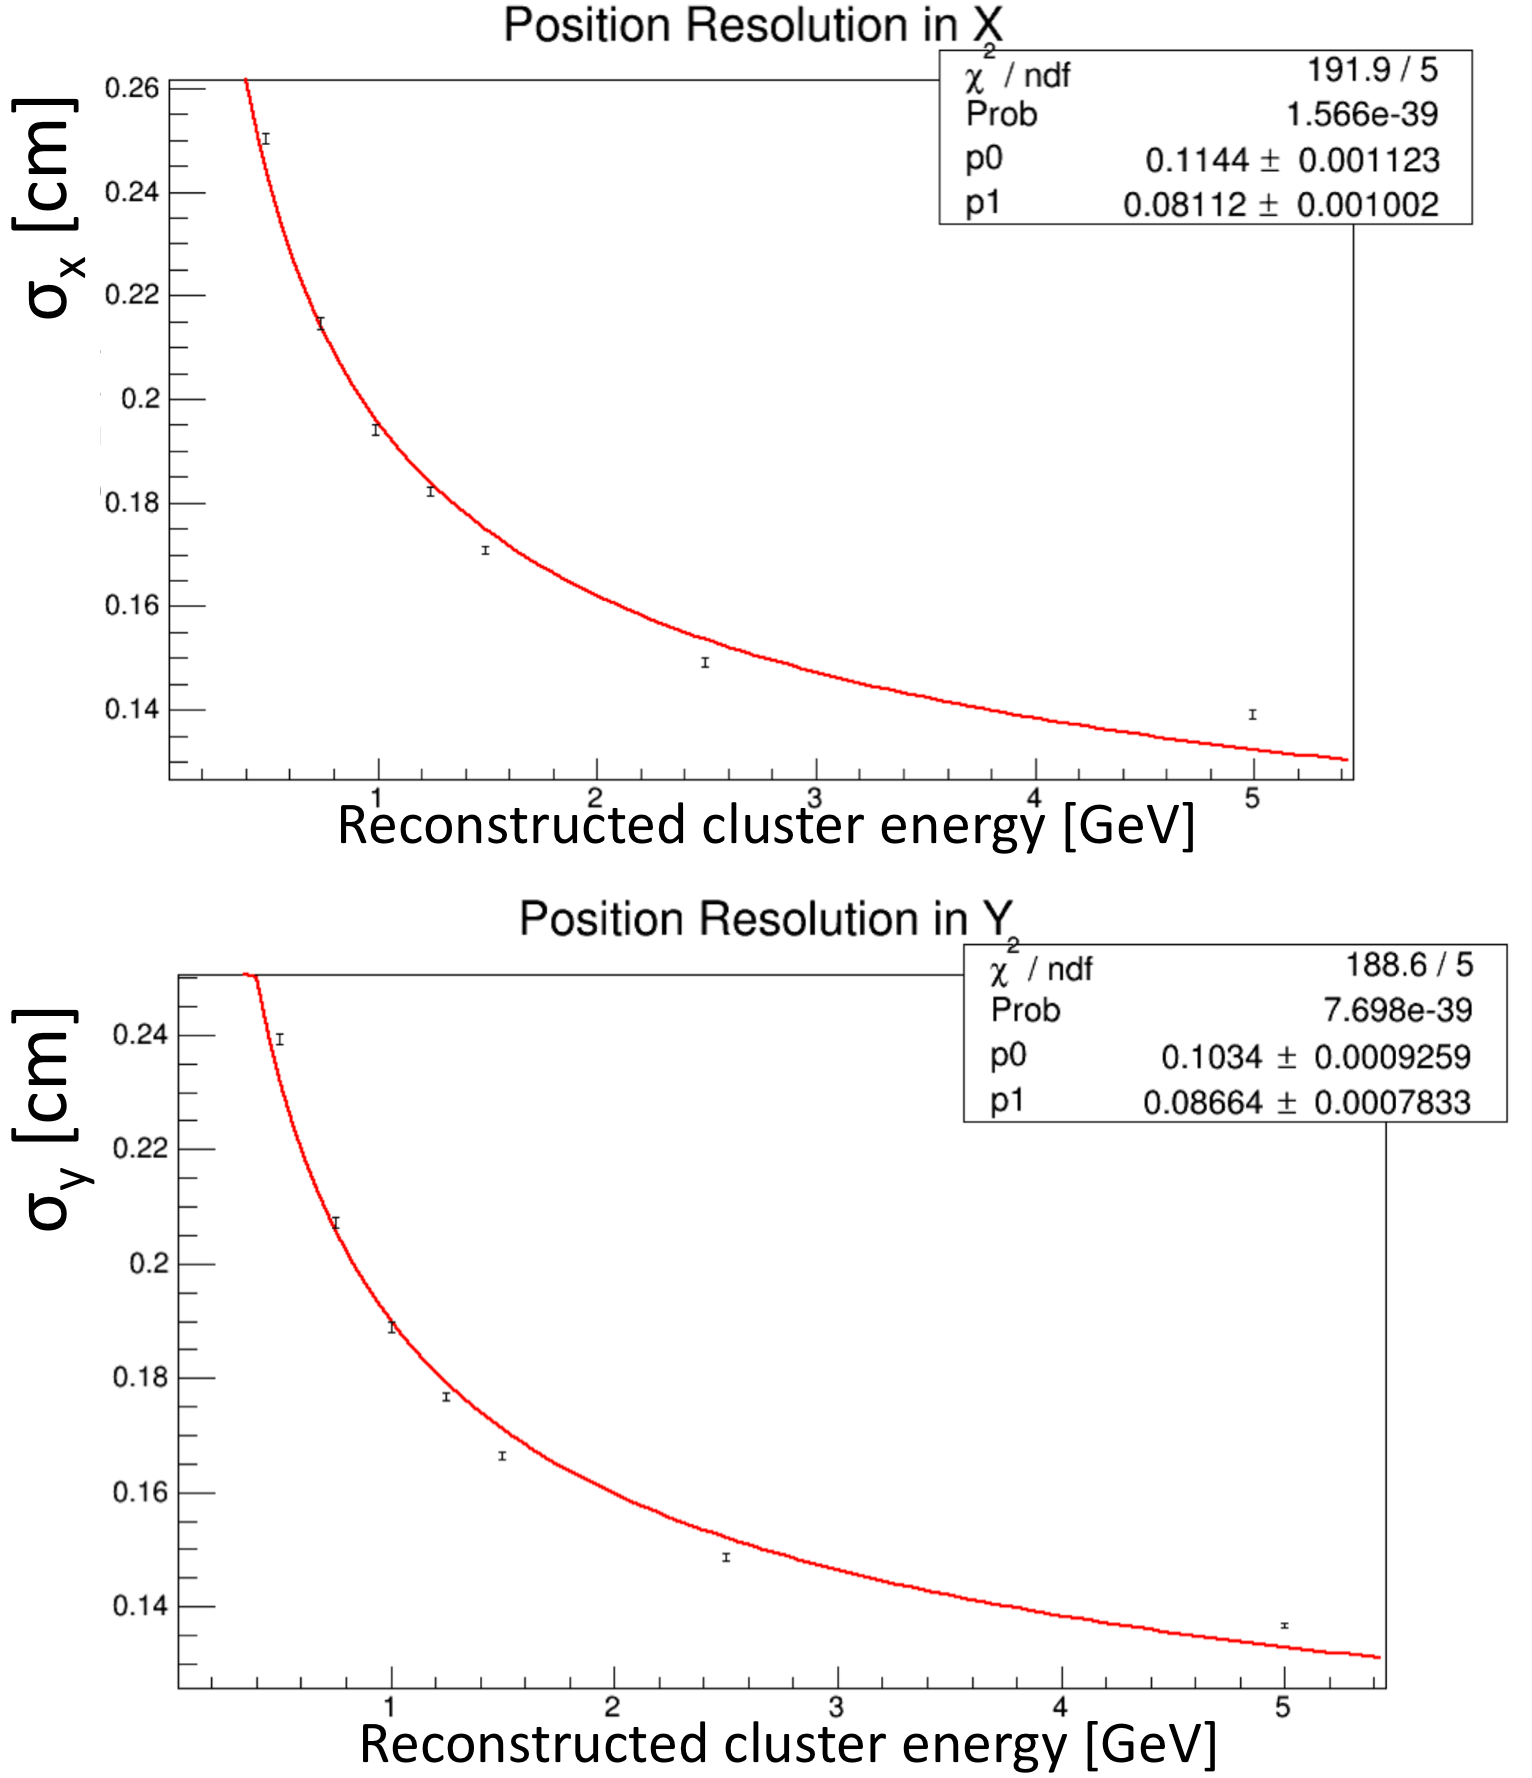
\includegraphics[width=0.7\textwidth]{pics/performance/emPosnResn.png}
  \caption[Energy-dependent position resolution for electrons.]{The energy-dependence of the position resolution for electrons as determined by me.}
  \label{Figure:emPosnResn}
\end{figure}

The position resolution is parameterized in terms energy following Equation~\eqref{eq:posnRes}.
 
\begin{equation}
\label{eq:posnRes}
\begin{split}
\sigma_x \textrm{[cm]}& =  \dfrac{p0_x}{\sqrt{E}}+p1_x\\
\sigma_y \textrm{[cm]}& =  \dfrac{p0_y}{\sqrt{E}}+p1_y
\end{split}
\end{equation}

The parameters $p0$ and $p1$ are found by fitting the residuals for the energies. The position resolution is better than 2~mm for 1~GeV electrons. As the ECal face is located at  approximately 1.4~m from the target, the ECal provides valuable position information when matched with a track. The position resolution for all particle types in the ECal is summarized in Table~\ref{tab:PosnResTable} as a function of $E_{rec}\textrm{[GeV]}$, where the reconstructed cluster energy is not corrected for shower-loss effects. 

\begin{table}[htb]
\caption{Position resolution.}
\label{tab:PosnResTable}
\centering
\begin{tabular}{|c|c|c|}
\toprule
%\multicolumn{2}{c}{Name} \\
%\cmidrule(r){1-2}
Particle & $\sigma_x$ [mm] & $\sigma_y$ [mm] \\
\midrule
electron & $0.1144/\sqrt{E_{rec}}+0.08112$ & $0.1034/\sqrt{E_{rec}}+0.08664$ \\
positron & $0.1268/\sqrt{E_{rec}}+0.07711$ & $0.1068/\sqrt{E_{rec}}+0.08423$ \\
photon & $0.1255/\sqrt{E_{rec}}+0.08877$ & $0.1005/\sqrt{E_{rec}}+0.08867$ \\
\bottomrule
\end{tabular}
\end{table}